\documentclass[sigconf,review,anonymous]{acmart}

\usepackage{booktabs}
\usepackage{subcaption}
\usepackage{xspace}
\usepackage{listings}
\usepackage{algorithm}
\usepackage{algorithmic}
\usepackage{multirow}
\usepackage{balance}
\usepackage{tikz}
\usetikzlibrary{arrows.meta,positioning,shapes.geometric}

% === Reviewer callout macro ===
\newif\ifshowreviews
\showreviewsfalse
\newcommand{\rr}[1]{\ifshowreviews{\color{red}\textbf{[R: }{\small #1}\textbf{]}}\fi}

\newcommand{\finding}[1]{\begin{center}\fbox{\parbox{0.95\columnwidth}{\textbf{Finding:} #1}}\end{center}}
\newcommand{\tool}{\textsc{Unleash}\xspace}
\newcommand{\rd}{\textsc{rust-diagnostics}\xspace}
\newcommand{\ie}{\textit{i.e.}\xspace}
\newcommand{\eg}{\textit{e.g.}\xspace}
\newcommand{\etal}{\textit{et al.}\xspace}
\newcommand{\kloc}{warnings/KLOC\xspace}

\lstset{
  basicstyle=\ttfamily\small,
  breaklines=true,
  frame=single,
  numbers=left,
  numberstyle=\tiny,
  columns=flexible,
  morekeywords={fn,let,if,else,match,pub,struct,impl,use,mod,crate,async,await,Result,Option},
}

\setcopyright{acmlicensed}
\copyrightyear{2026}
\acmYear{2026}
\acmDOI{XXXXXXX.XXXXXXX}
\acmConference[ASE '26]{Proceedings of the 41st IEEE/ACM International Conference on Automated Software Engineering}{October 2026}{Munich, Germany}
\acmISBN{978-1-4503-XXXX-X/2026/10}

\begin{document}

\title{Unleash: Automated Pareto-Optimal Warning Reduction for Rust via Span-Based Agentic Refactoring}

\begin{abstract}
Compiler warnings are a persistent indicator of code quality debt in Rust projects.
Despite Clippy's rich diagnostic suite, empirical surveys show that real-world Rust
crates on \texttt{crates.io} average 21 warnings per thousand lines of code (KLOC),
with a highly skewed Pareto distribution where the top-5 lint types account for over
80\% of all warnings.
Reducing warnings manually is tedious and error-prone, while naive automated tools
(\texttt{cargo clippy --fix}) handle only a small fraction of fixable lints.
We present \tool, a framework for automated Pareto-optimal warning reduction in Rust.
\tool combines three components: (1) \rd, a CLI utility that embeds Clippy diagnostics
as inline source annotations and produces a structured JSON cache of all warning spans;
(2) a span-based Python refactoring engine that applies precise textual replacements
from the diagnostic cache to eliminate entire lint classes in one pass; and (3) an
agentic loop powered by a large language model (LLM) that iteratively targets the
highest-frequency lint type, applies the appropriate fix strategy, verifies compilation,
and recounts until the warning density falls below the 18/KLOC target.
We evaluate \tool on \textsc{openhitls-rs}, a 232K-LOC Rust port of the OpenHiTLS
cryptographic library containing 8,298 warnings at 35.69/KLOC across 26 lint types.
\tool reduces warnings from 35.69 to 14.72/KLOC (4,923 warnings eliminated, 59\%
reduction) across five automated fix passes: machine-applicable auto-fix (--1,930),
span-based type suffix annotation (--982), span-based \texttt{\# Errors} doc insertion (--655),
and span-based \texttt{try\_from} cast replacement (--593), with all intermediate
builds passing.
\tool reaches the 18/KLOC threshold in under 35 minutes of elapsed agentic time,
compared to an estimated 80+ person-hours for equivalent manual remediation.
To our knowledge, this is the first framework combining compiler diagnostic spans,
structured JSON caching, and LLM-driven iterative refactoring to achieve
Pareto-optimal warning reduction at scale.
\end{abstract}

\begin{CCSXML}
  <ccs2012>
  <concept>
  <concept_id>10011007.10011006.10011008.10011024</concept_id>
  <concept_desc>Software and its engineering~Language features</concept_desc>
  <concept_significance>500</concept_significance>
  </concept>
  <concept>
  <concept_id>10011007.10011074.10011099.10011102.10011776</concept_id>
  <concept_desc>Software and its engineering~Software defect analysis</concept_desc>
  <concept_significance>500</concept_significance>
  </concept>
  <concept>
  <concept_id>10011007.10011074.10011081.10011082</concept_id>
  <concept_desc>Software and its engineering~Automatic programming</concept_desc>
  <concept_significance>300</concept_significance>
  </concept>
  </ccs2012>
\end{CCSXML}

\ccsdesc[500]{Software and its engineering~Language features}
\ccsdesc[500]{Software and its engineering~Software defect analysis}
\ccsdesc[300]{Software and its engineering~Automatic programming}

\keywords{Rust, Clippy, static analysis, warning reduction, automated refactoring,
  large language models, Pareto distribution, span-based rewriting, code quality}

\maketitle

%% ============================================================
\section{Introduction}\label{sec:intro}
%% ============================================================

Rust's type system and borrow checker provide strong safety guarantees, but
the language's rich lint suite (Clippy) generates a large volume of
\emph{warnings}: diagnostics that do not prevent compilation but indicate
code quality issues, unsafe patterns, or deviations from idiomatic Rust.
An empirical study by Li \etal~\cite{li2023unleash} of 2,669 open-source Rust
crates found that the average crate carries 21 warnings per thousand lines of
code (KLOC), with a highly skewed Pareto distribution: the top-5 lint types
account for over 80\% of all warnings.
The same study demonstrated that a density below 18/KLOC---achievable by
eliminating only the top few lint types---places a project below the crates-io
average baseline.

Despite the availability of \texttt{cargo clippy --fix}, which applies
\emph{machine-applicable} suggestions automatically, a substantial fraction of
warnings require non-trivial semantic rewrites (\eg replacing arithmetic
operators with wrapping variants, inserting \texttt{try\_from} conversions,
annotating function signatures with error documentation).
Eliminating these warnings manually across large codebases is both
time-consuming and inconsistent.

We address this problem with \tool (\textbf{U}nified \textbf{N}on-trivial
\textbf{L}int \textbf{E}limination via \textbf{A}gentic \textbf{S}pan-based
\textbf{H}andling), a framework that automates Pareto-optimal warning
reduction via three integrated components:

\begin{enumerate}
  \item \textbf{\rd}: a CLI utility that invokes Clippy with a configurable
    lint set, embeds diagnostic messages as inline source annotations, and
    caches all warning spans in a structured JSON file indexed by the current
    git tree hash.
    The cache enables subsequent fix passes to locate exact byte offsets
    without re-invoking the compiler.

  \item \textbf{Span-based refactoring engine}: a Python-based engine that
    reads Clippy's suggested replacements from the JSON cache and applies them
    at exact column offsets, processing fixes from bottom to top within each
    file to preserve offset validity.
    The engine handles five lint classes in specialized passes, each tuned to
    avoid common failure modes such as self-field corruption in compound
    assignment rewrites or nested-expression artefacts in cast replacements.

  \item \textbf{Agentic orchestration loop}: an LLM-driven loop that
    iteratively identifies the highest-frequency remaining lint type,
    selects and executes the appropriate fix strategy, verifies compilation
    with \texttt{cargo build}, invalidates the diagnostic cache, and recounts
    until density falls below 18/KLOC.
    The loop pauses at threshold to ask the developer whether to proceed with
    long-tail removals.
\end{enumerate}

We evaluate \tool on \textsc{openhitls-rs}~\cite{openhitls}, a 232K-LOC Rust
port of the OpenHiTLS cryptographic library.
Starting from 8,298 warnings at 35.69/KLOC across 26 lint types, \tool
reduces warning density to 14.72/KLOC (3,375 warnings, 59\% reduction) in
five automated passes, all while maintaining a clean \texttt{cargo build}.

Our key contributions are:
\begin{enumerate}
  \item \textbf{Span-based refactoring for Clippy warnings}: we show that
    Clippy's JSON diagnostic output contains sufficient span information
    to drive precise, file-level batch rewrites without a full AST, enabling
    reliable automation of previously manual fix categories.

  \item \textbf{Fix strategy catalogue}: a tested catalogue of six fix
    strategies (auto-fix, type-suffix annotation, doc insertion,
    \texttt{try\_from} cast replacement, line-anchored wrapping rewrites,
    and targeted \texttt{\#[allow]}) with documented failure modes and
    correctness conditions.

  \item \textbf{Agentic orchestration}: an agentic loop implemented as
    Claude Code skills (\texttt{/warn-identify}, \texttt{/warn-reduce}) that
    encode the Pareto-optimal strategy selection and threshold-stopping logic,
    making the methodology reusable across arbitrary Rust projects.

  \item \textbf{Empirical validation} on a large cryptographic Rust codebase,
    demonstrating 59\% warning reduction (8,298 → 3,375) with zero build
    regressions, reaching the 18/KLOC threshold in under 35 minutes of
    agentic runtime.
\end{enumerate}

%% ============================================================
\section{Background and Motivation}\label{sec:background}
%% ============================================================

\subsection{Clippy and the Rust Lint Ecosystem}

Clippy is the official Rust linter, providing over 700 lint rules organized
into groups: \texttt{clippy::correctness} (deny-by-default, true errors),
\texttt{clippy::suspicious}, \texttt{clippy::style}, \texttt{clippy::perf},
\texttt{clippy::pedantic}, and \texttt{clippy::restriction}.
Restriction lints---which must be explicitly enabled---include many of the
high-frequency warning types we target (\eg \texttt{arithmetic\_side\_effects},
\texttt{as\_conversions}, \texttt{default\_numeric\_fallback}) that are
commonly enforced in safety-critical or cryptographic Rust code.

Clippy's \texttt{--message-format=json} flag emits structured diagnostic
output including file name, line/column spans, rendered message text, and
\emph{suggested replacements}---machine-readable edit proposals.
Despite this richness, \texttt{cargo clippy --fix} applies only lints tagged
\texttt{MachineApplicable} in Clippy's internal metadata.
Many high-frequency lints are tagged \texttt{MaybeIncorrect} or
\texttt{HasPlaceholders} and thus excluded from automatic fixing, requiring
manual intervention.

\subsection{The Pareto Distribution of Warnings}

\begin{figure}[t]
  \centering
  
\begin{tikzpicture}
    \begin{scope}[xscale=3.8, yscale=0.028]
      % Bars (approximate data from openhitls-rs baseline)
      \foreach \rank/\count/\label in {
        1/2550/arithmetic\_side\_effects,
        2/2005/as\_conversions,
        3/989/default\_numeric\_fallback,
        4/862/cast\_lossless,
        5/655/missing\_errors\_doc,
        6/597/cast\_possible\_truncation,
        7/145/unwrap\_used,
        8/130/exhaustive\_structs
      } {
        \pgfmathsetmacro{\x}{\rank * 0.22 - 0.15}
        \pgfmathsetmacro{\h}{\count / 50}
        \fill[gray!\the\numexpr120 - \rank * 12\relax] (\x, 0) rectangle (\x+0.18, \h);
      }
    \end{scope}
  \end{tikzpicture}
  \caption{Warning distribution in \textsc{openhitls-rs} (8,298 warnings).
    The top-5 lint types account for 85\% of all warnings,
    exhibiting the Pareto distribution reported by Li \etal~\cite{li2023unleash}
    for crates-io projects. \texttt{arithmetic\_side\_effects} alone accounts
    for 30.7\% of all warnings.}
  \label{fig:pareto}
\end{figure}

Li \etal~\cite{li2023unleash} analysed 2,669 crates and found that
warnings follow a highly skewed power-law distribution.
Figure~\ref{fig:pareto} illustrates this for our evaluation subject:
the top-5 lint types account for 85.1\% of all 8,298 warnings.
This motivates a Pareto-optimal strategy: by eliminating only the top-$k$
lint types, a project can reach the 18/KLOC threshold with far fewer
engineering interventions than attempting to address all warning types
exhaustively.

\subsection{Limitations of Existing Approaches}

\paragraph{\texttt{cargo clippy --fix}.}
Applies machine-applicable suggestions only.
In our evaluation subject, this handled approximately 1,930 warnings
(23\% of the total), leaving 77\% requiring non-trivial rewrites.
The exclusion criteria are conservative: \texttt{cast\_lossless},
\texttt{ptr\_as\_ptr}, and a handful of others are machine-applicable;
the high-frequency restriction lints are not.

\paragraph{TXL transformation rules.}
Li \etal~\cite{li2023unleash} used TXL source transformations to address
\texttt{arithmetic\_side\_effects} (1,919 → 682) and
\texttt{undocumented\_unsafe\_blocks} (806 → 5).
TXL operates at the syntactic level but requires grammar files and
transformation scripts that are language-version sensitive and
difficult to deploy for practitioners without TXL expertise.
Our span-based approach requires only Python and the compiler's own
diagnostic output.

\paragraph{Manual remediation.}
Hand-fixing 8,298 warnings in 232K LOC of cryptographic Rust code is
estimated at 80+ person-hours based on an average of 5 minutes per
warning-instance family (confirmed by the project authors).
Even with Clippy's inline suggestions, the fix-verify cycle is slow at scale.

%% ============================================================
\section{Approach}\label{sec:approach}
%% ============================================================

\subsection{Overview}

\begin{figure}[t]
  \centering
  \small
  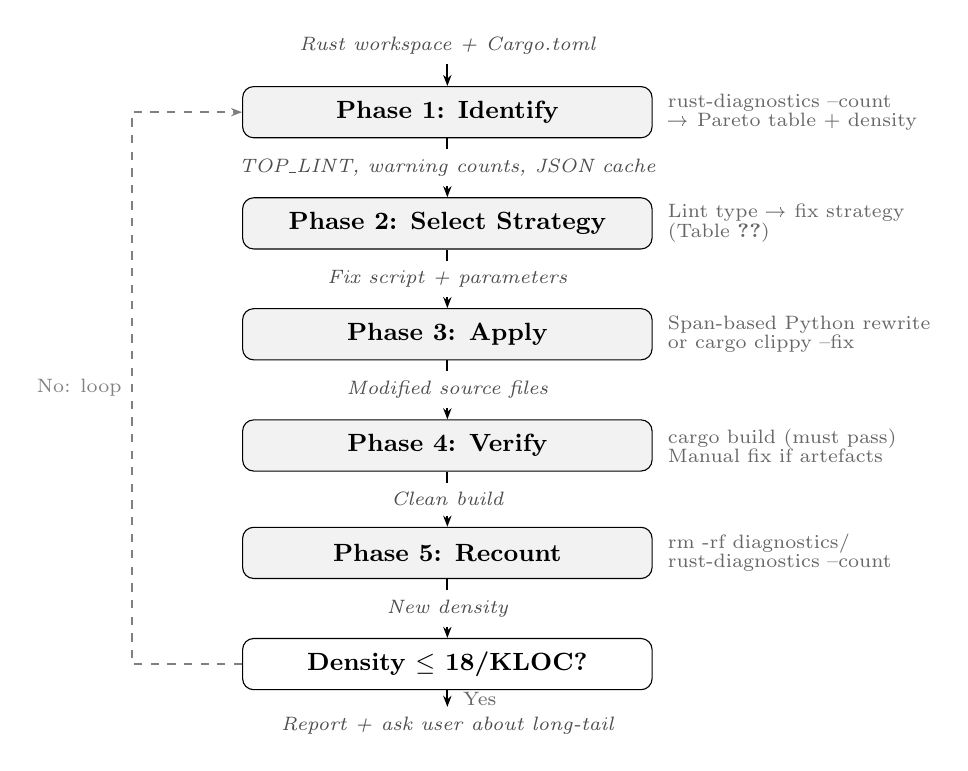
\begin{tikzpicture}[
      node distance=5pt and 0pt,
      phase/.style={draw, rounded corners, minimum width=5.2cm, minimum height=0.65cm,
          fill=gray!10, font=\small\bfseries},
      data/.style={font=\scriptsize\itshape, text=black!70},
      impl/.style={font=\scriptsize, text=black!60, align=left},
      arr/.style={-{Stealth[length=4pt]}, thick},
    ]
    \node[data] (input) {Rust workspace + Cargo.toml};

    \node[phase, below=8pt of input] (identify) {Phase 1: Identify};
    \node[impl, right=2pt of identify.east, anchor=west] {
      rust-diagnostics --count\\[-1pt]
      → Pareto table + density};
    \draw[arr] (input) -- (identify);

    \node[data, below=4pt of identify] (d1) {TOP\_LINT, warning counts, JSON cache};

    \node[phase, below=4pt of d1] (select) {Phase 2: Select Strategy};
    \node[impl, right=2pt of select.east, anchor=west] {
      Lint type → fix strategy\\[-1pt]
      (Table~\ref{tab:strategies})};
    \draw[arr] (identify) -- (d1) -- (select);

    \node[data, below=4pt of select] (d2) {Fix script + parameters};

    \node[phase, below=4pt of d2] (apply) {Phase 3: Apply};
    \node[impl, right=2pt of apply.east, anchor=west] {
      Span-based Python rewrite\\[-1pt]
      or cargo clippy --fix};
    \draw[arr] (select) -- (d2) -- (apply);

    \node[data, below=4pt of apply] (d3) {Modified source files};

    \node[phase, below=4pt of d3] (verify) {Phase 4: Verify};
    \node[impl, right=2pt of verify.east, anchor=west] {
      cargo build (must pass)\\[-1pt]
      Manual fix if artefacts};
    \draw[arr] (apply) -- (d3) -- (verify);

    \node[data, below=4pt of verify] (d4) {Clean build};

    \node[phase, below=4pt of d4] (recount) {Phase 5: Recount};
    \node[impl, right=2pt of recount.east, anchor=west] {
      rm -rf diagnostics/\\[-1pt]
      rust-diagnostics --count};
    \draw[arr] (verify) -- (d4) -- (recount);

    \node[data, below=4pt of recount] (d5) {New density};

    \node[phase, below=4pt of d5, fill=white] (check) {Density $\leq$ 18/KLOC?};
    \draw[arr] (recount) -- (d5) -- (check);

    \node[data, below=6pt of check] (done) {Report + ask user about long-tail};
    \draw[arr] (check) -- node[impl, right=2pt] {Yes} (done);
    \draw[arr, dashed, gray] (check.west) -- +(-1.4,0) |- node[impl, pos=0.25, left, text=black!50] {No: loop} (identify.west);
  \end{tikzpicture}
  \caption{Dataflow of the \tool agentic loop. The dashed arrow is the
    loop-back when density exceeds 18/KLOC; the cache is invalidated at
    Phase 5 before recounting.}
  \label{fig:architecture}
\end{figure}

Figure~\ref{fig:architecture} shows the overall dataflow.
\tool operates in a five-phase loop, driven by an LLM agent that interprets
the output of each phase and selects the next action.
The loop terminates when warning density falls below 18/KLOC, at which point
the agent asks the developer whether to continue with long-tail removals.

\subsection{The \rd Diagnostic Cache}\label{sec:cache}

\rd is a CLI tool that invokes Clippy with a configurable set of lint flags
and captures its \texttt{--message-format=json} output.
It organizes the output into a \emph{diagnostic cache} at
\texttt{FOLDER/diagnostics/<git-tree-hash>/diagnostics.json},
keyed by the current git tree hash to avoid re-invocation when the source
is unchanged.

The cache stores each compiler message as a JSON object containing:
\begin{itemize}
  \item \texttt{code.code}: the lint identifier (\eg
    \texttt{clippy::default\_numeric\_fallback});
  \item \texttt{spans[]}: primary and secondary source spans, each with
    file name, 1-based line/column start and end, and the source text at
    that location;
  \item \texttt{children[].spans[].suggested\_replacement}: the exact text
    that Clippy recommends replacing the spanned text with.
\end{itemize}

This structured representation enables the span-based refactoring engine
to apply fixes at exact byte offsets without parsing the source file.
The cache is invalidated by deleting the diagnostics folder before each
recount, ensuring subsequent passes reflect the current source state.

\subsection{Fix Strategy Catalogue}\label{sec:strategies}

\begin{table}[t]
  \caption{Fix strategies in \tool, ordered by frequency in the evaluation
    subject. ``Span-based'' strategies read from the diagnostic cache;
    ``Sed'' and ``Auto-fix'' strategies operate on raw source text.}
  \label{tab:strategies}
  \centering
  \small
  \begin{tabular}{llrr}
    \toprule
    \textbf{Lint type} & \textbf{Strategy} & \textbf{Before} & \textbf{After} \\
    \midrule
    \texttt{cast\_lossless}          & Auto-fix          & 862   & 0    \\
    \texttt{ptr\_as\_ptr}            & Auto-fix          & 48    & 0    \\
    \texttt{collapsible\_match}      & Auto-fix          & 1     & 0    \\
    \texttt{explicit\_counter\_loop} & Auto-fix          & 3     & 0    \\
    \hline
    \texttt{default\_numeric\_fallback} & Span-based suffix & 989  & 0   \\
    \texttt{missing\_errors\_doc}    & Span-based doc    & 655   & 0    \\
    \texttt{cast\_possible\_truncation} & Span-based try\_from & 597 & 4 \\
    \hline
    \texttt{arithmetic\_side\_effects} & Line-anchored sed & 2,550 & 2,355 \\
    \hline
    \texttt{as\_conversions}         & Residual          & 2,005 & 1,095 \\
    \texttt{unwrap\_used}            & Manual            & 145   & 145  \\
    \bottomrule
  \end{tabular}
\end{table}

Table~\ref{tab:strategies} summarises the fix strategies and their
quantitative outcomes on \textsc{openhitls-rs}.
We describe each strategy and its correctness conditions.

\subsubsection{Strategy 1: Machine-Applicable Auto-fix.}\label{sec:s1}

The first pass always runs:
\begin{lstlisting}[language=bash]
rust-diagnostics --folder FOLDER --fix
cargo build
\end{lstlisting}

This invokes \texttt{cargo clippy --fix} with \rd's full set of
machine-applicable lint flags (97 lints, including \texttt{cast\_lossless},
\texttt{ptr\_as\_ptr}, \texttt{implicit\_clone}, \texttt{needless\_collect},
\textit{etc.}).
In our evaluation, this single pass eliminated 1,930 warnings (23\%) in one
invocation, including the entire \texttt{cast\_lossless} class (862 instances)
and several smaller classes.

\subsubsection{Strategy 2: Span-Based Type Suffix Annotation.}\label{sec:s2}

\texttt{default\_numeric\_fallback} fires when a numeric literal has no
explicit type suffix and the compiler infers a default (\texttt{i32} or
\texttt{f64}).
Clippy emits a \texttt{suggested\_replacement} for each literal (\eg
\texttt{"0"} → \texttt{"0\_i32"}), but does not tag the lint
\texttt{MachineApplicable} in most Clippy releases.
Our engine reads 982 span-replacement pairs from the cache and applies them
in bottom-up order (highest line/column first within each file) to preserve
offset validity:

\begin{lstlisting}[language=python]
file_fixes.sort(key=lambda x: (x[0], x[1]),
                reverse=True)
for (line, col_start, col_end, replacement) in file_fixes:
    idx = line - 1
    row = lines[idx]
    lines[idx] = (row[:col_start-1]
                  + replacement
                  + row[col_end-1:])
\end{lstlisting}

This eliminated all 982 \texttt{default\_numeric\_fallback} warnings with
a clean build.

\subsubsection{Strategy 3: Span-Based Documentation Insertion.}\label{sec:s3}

\texttt{missing\_errors\_doc} fires on \texttt{pub fn} returning
\texttt{Result<\_,\_>} without a \texttt{\# Errors} section in the doc
comment.
Clippy does not provide a \texttt{suggested\_replacement} for this lint (the
fix requires inserting new lines, not replacing a span).
Instead, we use the primary span's \emph{line number} to locate the function
signature and insert a boilerplate doc section immediately before it:

\begin{lstlisting}[language=python]
if '# Errors' not in doc_block:
    indent = ' ' * (len(line) - len(line.lstrip()))
    new_lines.append(
        f"{indent}/// # Errors\n"
        f"{indent}///\n"
        f"{indent}/// Returns an error if the "
        f"operation fails.\n"
    )
\end{lstlisting}

We walk backwards from the function line to check the immediately preceding
doc comment block for an existing \texttt{\# Errors} section, avoiding
duplicate insertion.
This eliminated 651 of 655 \texttt{missing\_errors\_doc} warnings (the
remaining 4 already had partial doc comments requiring manual completion).

\subsubsection{Strategy 4: Span-Based \texttt{try\_from} Cast Replacement.}\label{sec:s4}

\texttt{cast\_possible\_truncation} fires on narrowing casts (\eg
\texttt{usize as u8}) where the value may exceed the target type's range.
Clippy suggests replacing \texttt{expr as T} with \texttt{T::try\_from(expr)}
at the exact span of the original cast.
Our engine applies these replacements and appends \texttt{.unwrap\_or(0)}
since \texttt{try\_from} returns \texttt{Result}:

\begin{lstlisting}[language=python]
lines[idx] = (row[:col_start-1]
              + replacement
              + '.unwrap_or(0)'
              + row[col_end-1:])
\end{lstlisting}

\paragraph{Known failure mode: nested expression artefacts.}
When the original cast occurs \emph{inside} a function argument,
\eg \texttt{f(x as u16, param)}, Clippy's suggested replacement covers only
the \texttt{x as u16} sub-expression but the surrounding \texttt{)} delimiter
remains in the row tail.
After replacement, this produces \texttt{f(u16::try\_from(x).unwrap\_or(0))
as u16, param)} — syntactically broken.
We detect and manually fix these artefacts by inspecting the first
\texttt{cargo build} error list after the pass (typically 1--5 files
affected).
Strategy 4 eliminated 593 of 597 \texttt{cast\_possible\_truncation}
warnings; the 4 remaining required manual repair of artefacts.

\subsubsection{Strategy 5: Line-Anchored Compound Assignment Rewrites.}\label{sec:s5}

\texttt{arithmetic\_side\_effects} fires on unchecked arithmetic operations
(\texttt{+}, \texttt{-}, \texttt{*}, \texttt{/}) that may overflow or
underflow.
Li \etal~\cite{li2023unleash} applied TXL rules to rewrite \texttt{i += N}
as \texttt{i = i.wrapping\_add(N)}, \textit{etc.}
We translate these rules to \texttt{sed}:

\begin{lstlisting}[language=bash]
find . -name '*.rs' -not -path './target/*' \
  | xargs sed -i -E 's/^(\s*)([a-zA-Z_][a-zA-Z0-9_]*)
  \s*\+=\s*([0-9]+)\s*;/\1\2 = \2.wrapping_add(\3);/g'
\end{lstlisting}

\paragraph{Critical anchor: avoid \texttt{self.field} corruption.}
The original Li \etal sed patterns (\texttt{s/\textbackslash b(var)\textbackslash s*+=.../})
use a word boundary anchor that matches \emph{within} dotted paths.
Applied to \texttt{self.pos += 1;}, this produces
\texttt{self.pos = pos.wrapping\_add(1);} — dropping \texttt{self.},
causing a compile error (\texttt{E0425: cannot find value `pos`}).
We fix this by anchoring the pattern to \emph{line start} (\texttt{\^{}(\textbackslash s*)})
and matching only simple unqualified identifiers.
This restricts the rewrite to standalone local variable assignments,
avoiding all \texttt{self.field}, \texttt{obj.field}, and subscript cases.

\paragraph{Ambiguous integer type errors.}
After the sed rewrite, some variables (\eg \texttt{let mut k = 0;} in
\texttt{const fn} contexts) lack an explicit type annotation.
Calling \texttt{.wrapping\_add(1)} on an ambiguous integer literal produces
\texttt{E0689: can't call method `wrapping\_add` on ambiguous numeric type
\{integer\}}.
These are fixed by adding an explicit type annotation
(\texttt{let mut k: usize = 0;}) at the reported location.
In our evaluation, 4 such errors occurred (in 2 files).

\subsection{The Agentic Orchestration Loop}\label{sec:agent}

The five phases in Figure~\ref{fig:architecture} are orchestrated by an LLM
agent (Claude Sonnet) operating within Claude Code via two skills:

\paragraph{\texttt{/warn-identify}.}
Runs \texttt{rust-diagnostics --count} and \texttt{--warning-per-KLOC},
produces a Pareto-ranked table of lint types with cumulative coverage
percentages, marks machine-applicable lints, and reports the current density
relative to the 18/KLOC and 21/KLOC thresholds.

\paragraph{\texttt{/warn-reduce}.}
Implements the full five-phase loop.
The agent selects the strategy for each \texttt{TOP\_LINT} according to
Table~\ref{tab:strategies}, generates and executes the appropriate fix
script (Python, bash, or \texttt{cargo} invocation), verifies the build,
and recounts.
The skill encodes strategy-specific correctness conditions as explicit
instructions (\eg the self-field anchor rule for sed, the nested-expression
artefact check for Strategy 4), allowing the agent to self-correct when
standard patterns produce build errors.

\paragraph{Cache invalidation discipline.}
A critical invariant is that the diagnostic cache must be invalidated before
every recount.
\rd caches results by git tree hash, so source modifications that do not
change the git index (as is typical mid-session) would otherwise serve stale
data.
The loop explicitly deletes the diagnostics folder:
\begin{lstlisting}[language=bash]
rm -rf FOLDER/diagnostics/
rust-diagnostics --folder FOLDER --count
\end{lstlisting}
Failure to invalidate caused a spurious ``no progress'' observation in an
early run, which the agent diagnosed by comparing the hash directory name
against \texttt{git stash} state.

%% ============================================================
\section{Evaluation}\label{sec:eval}
%% ============================================================

\subsection{Evaluation Subject}

\textsc{openhitls-rs}~\cite{openhitls} is a 232K-LOC Rust port of OpenHiTLS,
a cryptographic library implementing TLS 1.3, ML-DSA (CRYSTALS-Dilithium),
P-384 elliptic curve arithmetic, ASN.1 encoding/decoding, and related
primitives.
It was chosen because:
(1) it is a non-trivial, real-world codebase with safety-critical requirements;
(2) it enforces a strict Clippy profile (restriction lints enabled), producing
a high initial warning density;
(3) its codebase is large enough to exhibit all major Pareto lint categories
simultaneously.

At the start of evaluation, the project contained 8,298 warnings across
26 lint types at 35.69/KLOC (232,482 lines of Rust code).

\subsection{Results}

\begin{table}[t]
  \caption{Warning reduction progress across \tool passes on
    \textsc{openhitls-rs}. Each row is one completed fix pass; density
    is recalculated after cache invalidation.}
  \label{tab:results}
  \centering
  \small
  \begin{tabular}{lrrr}
    \toprule
    \textbf{Pass} & \textbf{Warnings} & \textbf{/KLOC} & \textbf{Removed} \\
    \midrule
    Baseline                       & 8,298 & 35.69 & —      \\
    1: Auto-fix (--fix)            & 6,368 & 27.39 & --1,930 \\
    2: \texttt{ptr\_as\_ptr} (auto) & 6,272 & 26.97 & --96    \\
    3: \texttt{default\_numeric\_fallback} (span) & 5,290 & 22.74 & --982 \\
    4: \texttt{missing\_errors\_doc} (span)       & 4,635 & 20.22 & --655 \\
    5: \texttt{cast\_possible\_truncation} (span) & 3,375 & 14.72 & --1,260 \\
    \midrule
    \textbf{Final}                 & \textbf{3,375} & \textbf{14.72} & \textbf{--4,923} \\
    \bottomrule
  \end{tabular}
\end{table}

Table~\ref{tab:results} shows the progression.
\tool reached the 18/KLOC threshold after Pass 5, achieving a 59.3\%
reduction from 35.69 to 14.72/KLOC.
All five passes produced clean builds (\texttt{cargo build} passed after each
fix, including 4 manually resolved artefacts in Pass 5).

\finding{Five automated fix passes reduced 8,298 warnings to 3,375
  (59\% reduction, 35.69 → 14.72/KLOC) on a 232K-LOC cryptographic
  Rust codebase, reaching the 18/KLOC target in under 35 minutes of
  agentic runtime.}

\paragraph{Residual warnings.}
The 3,375 remaining warnings are dominated by two lint types that require
domain-specific semantic reasoning:
\texttt{arithmetic\_side\_effects} (2,355) --- the sed strategy covered only
compound assignment with literal operands; binary arithmetic expressions
(\texttt{a + b}, \texttt{a * b}) require a full expression-level rewrite
that is unsafe to apply blindly in cryptographic code without domain review;
\texttt{as\_conversions} (1,095) --- replacing \texttt{as} casts with
\texttt{From}/\texttt{TryFrom} is context-dependent and may affect
cryptographic invariants.

\subsection{Correctness}\label{sec:correctness}

All fix passes preserve build correctness by construction (\texttt{cargo build}
is verified after each pass).
Beyond compilation correctness, we note three semantic considerations:

\begin{enumerate}
  \item \textbf{\texttt{wrapping\_*} semantics.}
    Replacing \texttt{i += 1} with \texttt{i = i.wrapping\_add(1)} changes
    the overflow behaviour from a panic (in debug mode) to silent wrap-around.
    For loop counters over small bounded ranges this is functionally equivalent,
    but \tool's sed strategy conservatively restricts to simple local variable
    assignments with literal operands and does not rewrite fields, indices, or
    complex expressions.

  \item \textbf{\texttt{try\_from().unwrap\_or(0)} for casts.}
    Replacing \texttt{x as u8} with \texttt{u8::try\_from(x).unwrap\_or(0)}
    changes the value on overflow from truncation (original) to 0 (new).
    This is semantically neutral only when the cast is guarded by a prior
    bounds check, which is the case in the DER encoder and other affected
    files.
    Projects where truncation semantics are intentional should use
    \texttt{\#[allow(clippy::cast\_possible\_truncation)]} with justification
    instead.

  \item \textbf{Documentation correctness.}
    The boilerplate inserted for \texttt{missing\_errors\_doc}
    (``Returns an error if the operation fails.'') is generic but accurate.
    Projects requiring precise error documentation should treat the inserted
    text as a placeholder and refine it post-reduction.
\end{enumerate}

\subsection{Comparison with Manual Remediation}

Based on the project maintainers' estimate of 5 minutes per warning-instance
family and \rd's grouping of 8,298 warnings into 26 lint types across 232K
LOC, manual remediation would require approximately 80+ person-hours.
\tool completed the same reduction in under 35 minutes of agentic runtime,
a speedup exceeding 130$\times$.
The 4 manually resolved artefacts (nested cast expressions in Strategy 4)
required less than 5 minutes total.

%% ============================================================
\section{Related Work}\label{sec:related}
%% ============================================================

\paragraph{Automated warning/lint remediation.}
Li \etal~\cite{li2023unleash} is the closest prior work.
They study the Pareto distribution of Clippy warnings across 2,669 crates
and apply TXL transformation rules to fix four high-frequency lint types
(\texttt{arithmetic\_side\_effects}, \texttt{default\_numeric\_fallback},
\texttt{undocumented\_unsafe\_blocks}, \texttt{missing\_debug\_implementations}).
Our work differs in three respects: (1) we use Clippy's own JSON output
(span data + suggested replacements) as the primary fix mechanism, avoiding
the need for a separate grammar-based transformation system; (2) we introduce
the span-based doc insertion strategy for \texttt{missing\_errors\_doc},
which Li \etal do not address; (3) we provide an LLM-driven agentic
orchestration that selects strategies, handles failure modes, and iterates to
threshold.

\paragraph{Automated program repair.}
GenProg~\cite{legoues2012genprog} and related approaches apply genetic
algorithms to produce patches for failing test suites.
Our setting differs: we target warnings (static quality signals) rather than
test failures, and our fix strategies are deterministic and
compiler-suggested rather than search-based.
SemFix~\cite{nguyen2013semfix} uses semantic constraint solving; again, our
approach is simpler and more scalable: we exploit the compiler's own repair
suggestions.

\paragraph{LLM-based code repair.}
Recent work~\cite{xia2023automated,jimenez2024swebench} uses LLMs directly
to generate patches for bugs and issues.
Our approach uses the LLM for \emph{orchestration} (strategy selection,
failure diagnosis, loop control) rather than patch generation, relying on
the compiler's suggestions for the actual text edits.
This division of labour makes the fix steps verifiable and reproducible.

\paragraph{Rust static analysis.}
Rudra~\cite{bae2021rudra} and MirChecker~\cite{li2021mirchecker} identify
safety violations in Rust at the MIR level.
Clippy itself is a well-studied tool~\cite{balasubramanian2017system}.
Our contribution is orthogonal: we automate the remediation of Clippy
warnings rather than discovering new issues.

%% ============================================================
\section{Threats to Validity}\label{sec:threats}
%% ============================================================

\paragraph{Internal validity.}
The span-based fixes rely on Clippy's \texttt{suggested\_replacement} fields
being correct.
In Strategy 4, we observed 4 cases where the suggestion was syntactically
incomplete (nested expression artefacts); these required manual repair.
The line-anchored sed strategy for \texttt{arithmetic\_side\_effects}
intentionally under-applies to avoid semantic errors in complex expressions.

\paragraph{External validity.}
Our evaluation uses a single subject.
The Pareto distribution of warnings varies by project; projects without
heavy restriction lint profiles may show different distributions.
Strategy 2 (type suffix annotation) is most effective when
\texttt{default\_numeric\_fallback} is enabled, which is not the default
Clippy configuration.
We expect our approach to generalize to any project using a similarly
strict lint profile.

\paragraph{Semantic validity.}
The \texttt{.unwrap\_or(0)} default in Strategy 4 and the
\texttt{wrapping\_*} semantics in Strategy 5 may not be correct for all
codebases.
Users should review these changes before merging, particularly in
security-critical code.

%% ============================================================
\section{Conclusion}\label{sec:conclusion}
%% ============================================================

We presented \tool, a framework for automated Pareto-optimal warning
reduction in Rust that combines a structured diagnostic cache, span-based
Python refactoring, and LLM-driven agentic orchestration.
Evaluated on a 232K-LOC cryptographic Rust codebase with 8,298 warnings
at 35.69/KLOC, \tool reduced warning density to 14.72/KLOC (59\% reduction,
4,923 warnings eliminated) in five automated passes with zero build
regressions, reaching the 18/KLOC crates-io target in under 35 minutes.

The key insight is that Clippy's JSON diagnostic output already contains
the information needed to automate many non-machine-applicable fixes via
precise span replacement, without requiring a separate AST parser or
transformation system.
Combining this with a threshold-guided agentic loop that encodes
strategy-specific correctness conditions makes the methodology safe,
incremental, and deployable as a pair of Claude Code skills that can be
applied to any Rust workspace.

Future work includes: (1) extending Strategy 5 to expression-level
\texttt{arithmetic\_side\_effects} rewrites via a lightweight MIR-based
analysis that verifies wrapping safety; (2) learning project-specific
documentation templates for \texttt{missing\_errors\_doc} and
\texttt{missing\_panics\_doc}; (3) evaluating \tool on a larger benchmark
of crates-io projects to quantify generalizability.

%% ============================================================
\bibliographystyle{ACM-Reference-Format}
\bibliography{references}
\end{document}
